
The growing disparity in income and opportunities across the US is becoming one of the most pressing issues of modern society. The complexity of both causes and consequences has been faced with a wide spectrum of both \textit{place-} and \textit{person-based} policy tools, but what are the the first-order impacts of many of them is still an open question. Focusing on the former, in recent years many US jurisdictions have adopted minimum wage laws (hereafter MW) setting workers' hourly pay above the federal minimum of \$7.25.\footnote{As of January 2020, there were 29 states with a minimum wage higher than the federal one, 52 counties with a MW above the state's, and 15 cities with a MW above the county's.} Despite a prominent debate around recent MW policies both at local and national level, starting from the seminal work of \textcite{card2000minimum}, most research effort has been directed towards understanding the effects of MW on employment \parencite[e.g,][]{dube2010minimum, neumark2006minimum, cengiz2019effect}. This is not surprising, as employment effects are of first order importance to understand the welfare implications of MW changes. However, as non-federal MW changes are \textit{place-based} by definition, it is also natural to expect these changes affecting households' welfare through markets other than the labor one. A very likely candidate to experience such effects is the housing market: How do local rents and prices react to MW changes? Surprisingly, there is very little research estimating the effects of MW on rents and house values, and virtually no research estimating the effects on local amenities.\footnote{To our knowledge the only papers aiming at answering this question are \textcite{yamagishi2019minimum} and \textcite{tidemann2018mw}. Surprisingly, they both found opposing results despite using the same year-county data. \textcite{yamagishi2019minimum} find a small positive effect, while \textcite{tidemann2018mw} finds a small negative effect. \textcite{yamagishi2019minimum} attributes this difference to different model specifications, and argues that with proper standard errors clustering the results in \textcite{tidemann2018mw} are statistically insignificant. We will soon explain the differences of this paper with those.} We argue that estimates of these effects are crucial to pin down the welfare consequences of changes in the minimum wage, even more as MW policies have been increasing adopted at the county and city level.

In support to the previous motivation, we plot in In \autoref{fig:binsc_rent_mwpctchange} the binned correlation between the zipcode level median rent for single family homes and condos (sfcc) and the previous year's percentage change in the binding MW, while controlling for year yearly averages and socio-economic demographics. The positive relationship is clearly visible, and it looks slightly quadratic suggesting that indeed we do observe the expected relationship between our measures of interest. We replicate this exercise for median listing prices (\autoref{appfig:binsc_listing_mwpctchange}), and we also find a clear positive relationship. 

\begin{figure}[htb]
    \centering
    \caption{Correlation Between Median Rent Price (in dollars per square foot) and previous year change in MW (percentage).}
    \scalebox{0.20}{
    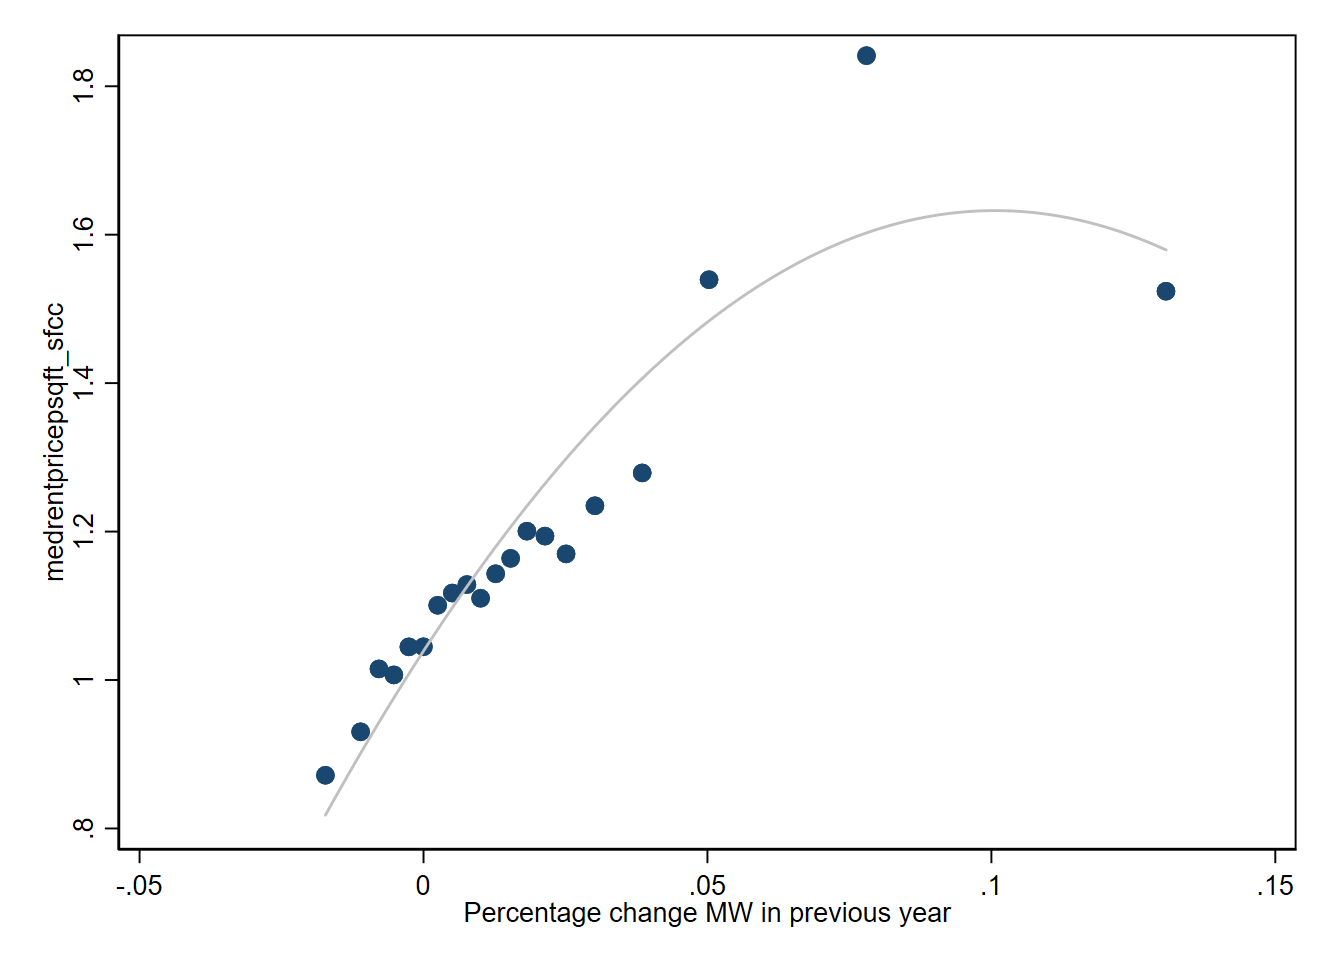
\includegraphics{draft_june20/tempfigure/binsc_medrentpricepsqft_sfcc_pctMWch.png}}
    \subcaption*{\textit{Note}: The figure presents the correlation between median rent price on zillow.com at the zipcode-year level and the percentage change in MW in the previous year. Data comes from the final sample used in the analysis (see \autoref{sec:data} for more details). Each zipcode yearly observation is obtained by averaging monthly observations, the basic time unit in this paper. The correlation is taken after controlling for year fixed effects, resident population, urban share, median income, black population share, and number of housing units.All demographic characteristics come from the 2010 Census.   
    }
    \label{fig:binsc_rent_mwpctchange}
\end{figure}




% I think next paragraph is unnecessary

%A canonical version of the Alonso-Muth-Mills model with homogeneous agents predicts that wage increases should be fully capitalized by landlords, as workers end up paying higher rents in all locations.\footnote{See \textcite{brueckner1987structure} for a complete treatment of the Alonso-Muth-Mills model.} A 1-to-1 pass-through is clearly a consequence of the strong assumptions embedded in that model, such as homogeneity of agents and perfectly-elastic housing market. Alternative city-level models, such as \textcite{klinemoretti2014}, suggest that an increase of the wage in one location would increase both population and rents, although with a smaller pass-trough. \textcite{yamagishi2019minimum} shows one example where, due to the increased probability of unemployment after a MW increase, the effect of the MW on rents is ambiguous --although positive if there are no disemployment effects. We will develop a theoretical model to discuss this question, and we will further include amenities into it. We hypothesize that a MW increase in a location can have effects that go way beyond traditional ``labor market'' outcomes. As emphasized by recent research \parencite[e.g.,][]{diamond2016determinants}, accounting for both rents and amenities is crucial to understand changes in welfare.
 
In this paper, we use data at the zipcode-month level to assess the reduced form effects of MW changes on rents, house values, and amenities. In the future, we hope to develop a spatial equilibrium model with agents that trade-off wages and amenities heterogeneously.\footnote{We are currently working on this model.} The model we have in mind has two types of agents (high and low) who choose where to locate among many discrete locations. We want to derive theoretical predictions on equilibrium rents and amenities when we change exogenously the wage of the low type workers in some locations and not in others. We also have in mind to extend the model to allow for different land availability in different locations, as places we expect locations with tighter land availability to have bigger rent increases than locations with more available land (and therefore with a more elastic housing supply). 

Estimating empirically the pass-through from MW to rents is not only policy relevant, but is also of theoretical interest. As shown by \textcite{agarwal2019minimum}, if landlords know that their tenants have more disposable income raising the rent will have two theoretical effects. On one hand, it increases the landlords revenue conditional on receiving the rent payment. On the other hand, it increases the probability of tenants defaulting their payment. 

From an estimation perspective, one of the main challenge to correctly identify the pass-through to rents and house prices is to isolate exogenous variations in the MW: determinants of the MW are likely to be correlated with geographical and time factors also affecting the housing market in a direct way. 
 
To overcome this challenge, we use a panel event-study methodology \parencite{abraham2018estimating, BorusyakJaravel2017} at the zipcode-month level exploiting the fine timing of hundreds of MW changes across different US jurisdictions from 2010 to 2019. As the MW changes are staggered across zipodes and dates, we estimate the relevant pass-through by leveraging on within zipcode variation around the relative time of the event while we control for geographic and geographic-specific time fixed effects. This yields the causal effect assuming that factors leading to MW changes are not related to unobservable factors affecting housing market outcomes. Although we cannot directly test that assumption, in practice, the usual way of assessing its plausibility is by making sure that pre-event coefficients in the event-study regression show no trend.\footnote{Recent work by \textcite{roth2018pre} has developed methods to integrate pre-trend testing into the design to get correct standard error coverage.}. In addition, pooling hundreds of MW changes in an event study is more likely to be externally valid than research based on a few case studies. \\

[ADD RESULTS] \\

\paragraph{Related Literature.}
Our approach has several differences with respect to past papers. Both \textcite{tidemann2018mw} and \textcite{yamagishi2019minimum} use Fair Markets Rents data which is available at the year-county level.\footnote{\textcite{yamagishi2019minimum} also uses data at the year-prefecture level for the 47 Japanese prefectures.} An important advantage of our approach is that we use the exact timing of the MW change at the monthly level. When using variation at the year level the event period is "partially treated" which will tend to understate the magnitude of the effect. Furthermore, some jurisdictions have MW changes on many subsequent years, making it challenging to estimate the dynamics around changes that are followed by changes in the immediate year. For example, if there is a change in two subsequent years, then the estimated effect of the change in the second year may be due too the effect of the current MW change or to the past MW change or both.

Furthermore, we use data at the zipcode level instead of at the county.\footnote{As of 2019 there were 3142 counties and 39295 meaningful zipcodes\footnote{We exclude military and unique business zipcodes as they are irrelevant for house prices.} in the US.} To illustrate why this is important think about the following example. For simplicity suppose that in a certain county, just before a MW change, all low skill jobs are in one particular zipcode. Suppose further that low skill households prefer to live near their jobs and the MW increases. Suppose, consistently with \textcite{card2000minimum} and \textcite{cengiz2019effect}, that employment effects are near zero. Then, one should expect demand for housing in the zipcode with the low skill jobs to increase and demand for housing in the rest of the zipcodes to go down. If we focus, on the effects of the MW increase on the county we might even find that the rents go down, when in fact the rents in the zipcodes were the low skill jobs are will increase. Indeed, \textcite{tidemann2018mw} found that a \$1 increase in the MW decreases the yearly average of the monthly rent by 1.5 percentage points\footnote{As pointed out by \textcite{tidemann2018mw}, the sign of this effect implies that the labor demand for low skilled workers is elastic. This is at odds with the results from \textcite{card2000minimum}, \textcite{cengiz2019effect}, and many others.}. If we add amenities to the example, matters become much more complicated but if we allow for high skill people to value amenities differently than low skill people (like in \textcite{diamond2016determinants}), we may also expect to see residential resorting of high skill people depending on where are the amenities located, whether the amenities respond endogenously to the high-low skill composition of the zipcode, and depending on which are the zipcodes that the low skilled workers are demanding less. This example, illustrates that as the spatial distribution of jobs and amenities varies at the very local level, when tastes are heterogeneous by skill (or some other dimension) focusing on a large geographic area may be misleading. A second advantage of having a more detailed geography is that we can use census to compute the level of employment and the distribution of income in each zipcode, and check if we observe stronger effects on rents in places where there are more MW earners or in places where there is more low skilled employment. 
A third important difference of our approach is that by exploiting data at the zipcode-month level we can test the robustness of the event study design well beyond two-way county-year fixed effects. Our baseline specification has zipcode fixed effects, state-specific year-month fixed effects, and county-specific calendar-month fixed effects that allow for very flexible seasonal patterns. This in turn has two important advantages. First, it makes our estimates much more precise than the previous ones. Second, and most important, it makes substantially more plausible the needed identification assumptions. Given that the identifying variation comes from within zipcodes, the determinants of these MW changes are unlikely to be related to the zipcode, and therefore, are less likely to be correlated to the unobservable determinants of rents in that zipcode.

A fourth important difference with the past work, is that to the best of our knowledge, this is the first study that estimates the effect of MW changes on amenities. As pointed out recently by \textcite{diamond2016determinants, almagro2019location}, taking into account non-pecuniary dimensions of the utility function can change substantively the welfare computations and the incidence of policy relevant changes. We exploit the use of high frequency GPS data to build amenity measures at the zipcode-month level and estimate the effect of MW changes on them. We hope that by incorporating amenities into the picture we can give a more comprehensive assessment of the effects of MW policies.

Another difference with the past work is that, given the spatial granularity of our data, we can use MW changes at any jurisdictional level (national, state and local). This is interesting because MW changes at different jurisdiction levels may have different local effects on rents. Intuitively, this is the case because, for example, out-of-state migration is in principle more costly than out-of-county migration, therefore, we expect more residential resorting within a state and across counties when a county changes their local MW wage. Our data allows us to study the heterogeneous effects of different MW changes.\footnote{In principle, our data allows us to answer whether the effects of changes at the federal, state, county, and city/town level are different.} 

Beyond the contribution to the very recent literature on the effects of MW changes on rents, we contribute to several strands of the literature. First, we contribute to the literature studying the effects of minimum wages on the welfare of low skill households. However, instead of focusing on wages and employment\parencite{dinardo1995labor, autor2016contribution, card2000minimum, neumark2006minimum, jardim2017minimum}, we contribute to this strand by taking into account the effects on the housing market.

Second, our work relates to the literature that studies the location decision of agents either based on income \parencite{roback1982wages, kennan2011effect, desmet2013urban, perez2018city} or based on spatial rent and amenity differentials \parencite{diamond2016determinants,almagro2019location,couture2019income, bayer2004equilibrium}. We hope to contribute by adapting this framework to the case of the MW changes, so that we can rationalize through residential location sorting part of the observed reduce form effect on rents and amenities. 

% incorporates the response of spatially differentiated amenities into place, in particular 